\clearpage
\section{Monopolistická konkurence (charakteristiky, krátkodobá rovnováha firmy,
dlouhodobá rovnováha firmy)}

\subsection{Charakteristiky monopolistické konkurence}
\begin{itemize}
    \item Mnoho firem
    \item Podobné, ale diferencované statky (např. mobilní telefony), jsou to vzájemné substituty
    \item Nízké bariéry vstupu do odvětví
    \item Žádná firma nemá dominantní postavení
\end{itemize}

\subsection{Krátkodobá rovnováha firmy}
\begin{itemize}
    \item Opět se vychází z $MR=MC$, z toho se zjistí objem a cena se dopočítá podle poptávkové křivky.
    \item $AR>AC$, monopolní zisk existuje
\end{itemize}
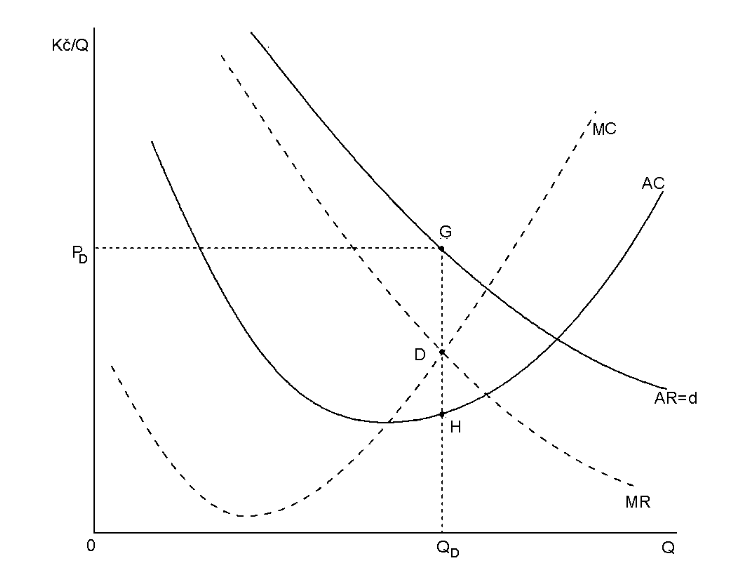
\includegraphics[width=16cm]{images/15_kratkodobe.png}

\subsection{Dlouhodobá rovnováha firmy}
\begin{itemize}
    \item Směřuje k nulovému monopolnímu zisku, protože vstupní náklady jsou nízké
    \item $AR\approx AC$
\end{itemize}
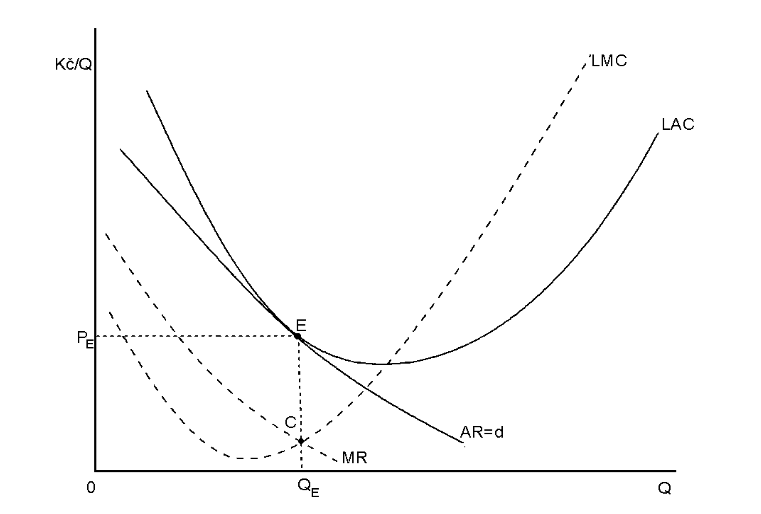
\includegraphics[width=16cm]{images/15_dlouhodobe.png}